\chapter{Introduzione}

Una \textbf{base di dati} è un insieme organizzato di dati utilizzati per il supporto allo svolgimento di attività (di un ente, azienda, ufficio, persona).

Le figure coinvolte nella costruzione di una base di dati sono:
\begin{itemize}
	\item Committente:\ dirigente, operatore.
	\item Fornitore:\ direttore del progetto, analista, progettista di BD, programmatore di applicazioni che usano BD.
	\item Manutenzione e messa a punto della BD/Gestione del DBMS:\ amministratore del DBMS.
\end{itemize}

\section{Sistemi informativi}

\begin{definition}
	Un \textbf{sistema informativo} di un'organizzazione è una combinazione di risorse, umane e materiali, e di procedure organizzate per la raccolta, l'archiviazione, l'elaborazione e lo scambio delle informazioni necessarie alle attività operative (informazioni di servizio), di programmazione e controllo (informazioni di gestione) e di pianificazione strategica (informazioni di governo).
\end{definition}

\section{Sistemi informatici}

Il \textbf{sistema informativo automatizzato} è quella parte del sistema informativo in cui le informazioni sono raccolte, elaborate, archiviate e scambiate \textit{usando un sistema informatico}.

Il \textbf{sistema informatico} è l'insieme delle tecnologie informatiche e della comunicazione (Information and Communication Technologies, ICT) a supporto delle attività di un'organizzazione.

\begin{figure}[H]
	\centering
	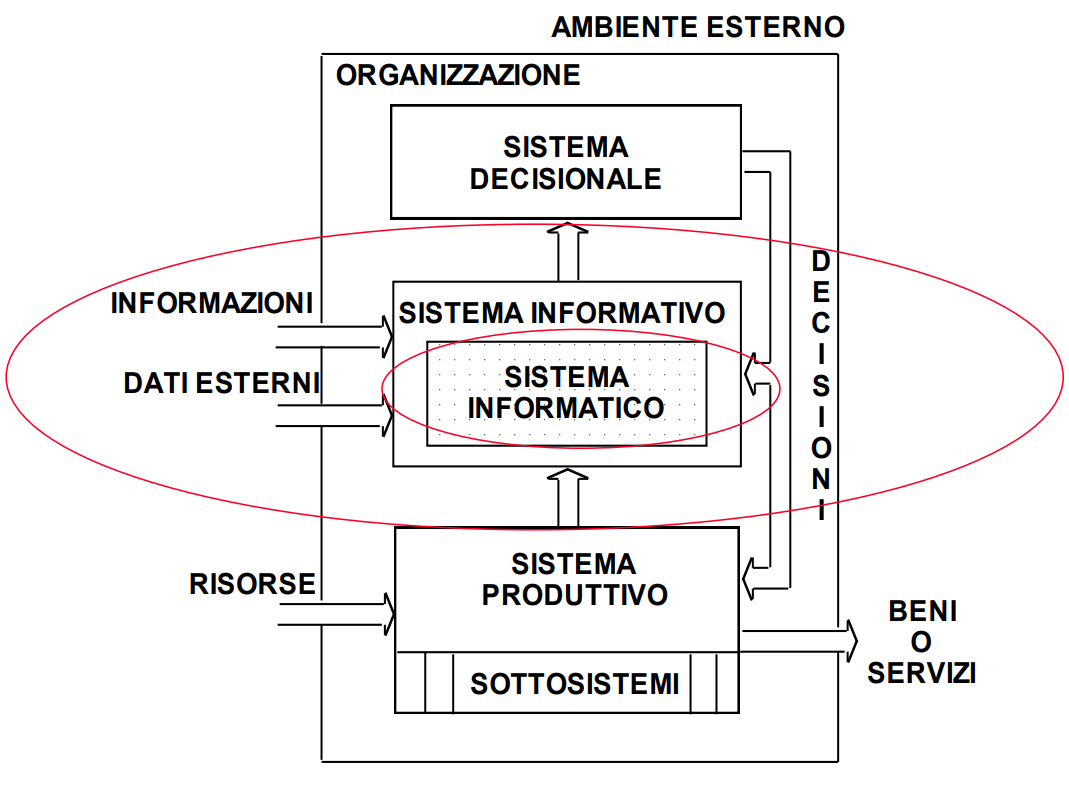
\includegraphics[width=0.8\textwidth]{immagini/Sistemi_informatici.png}
	\caption*{Sistema informatico nelle organizzazioni}
\end{figure}
\noindent Terminologia:
\begin{itemize}
	\item sistema informativo $\approx$ sistema informativo automatizzato
	\item sistema informativo automatizzato $\approx$ sistema informatico
\end{itemize}

\begin{figure}[H]
	\centering
	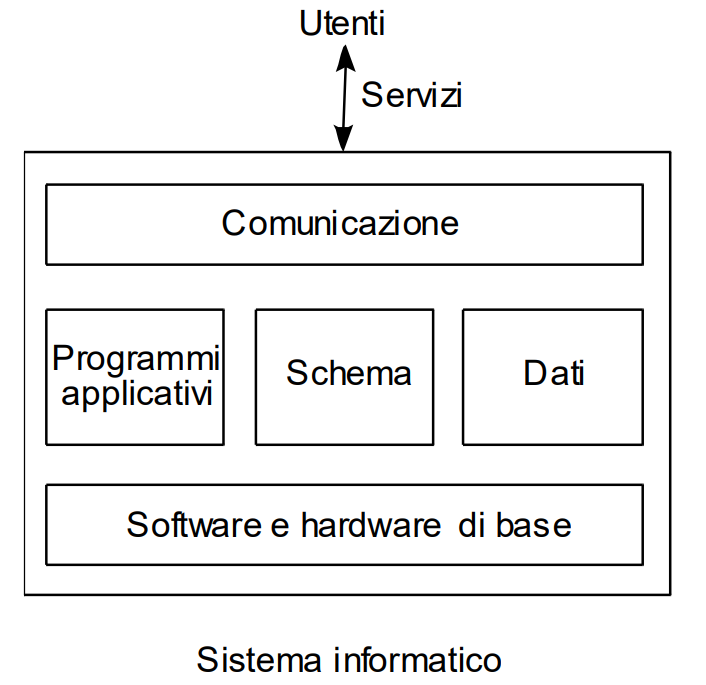
\includegraphics[width=0.4\textwidth]{immagini/Sistema_informatico.png}
	\caption*{Componenti di un sistema informatico}
\end{figure}
\subsection{Sistemi informatici operativi}
I dati sono organizzati in basi di dati.\
Le applicazioni si usano per svolgere le classiche \textbf{attività strutturate e ripetitive dell'azienda} nelle aree amministrativa e finanziaria, vendite, produzione, risorse umane, \dots

Le caratteristiche delle basi di dati sono garantite da un sistema per la gestione di basi di dati (\textbf{Data Base Management System}, \textbf{DBMS}), che ha il controllo dei dati e li rende accessibili agli utenti autorizzati.

\begin{figure}[H]
	\centering
	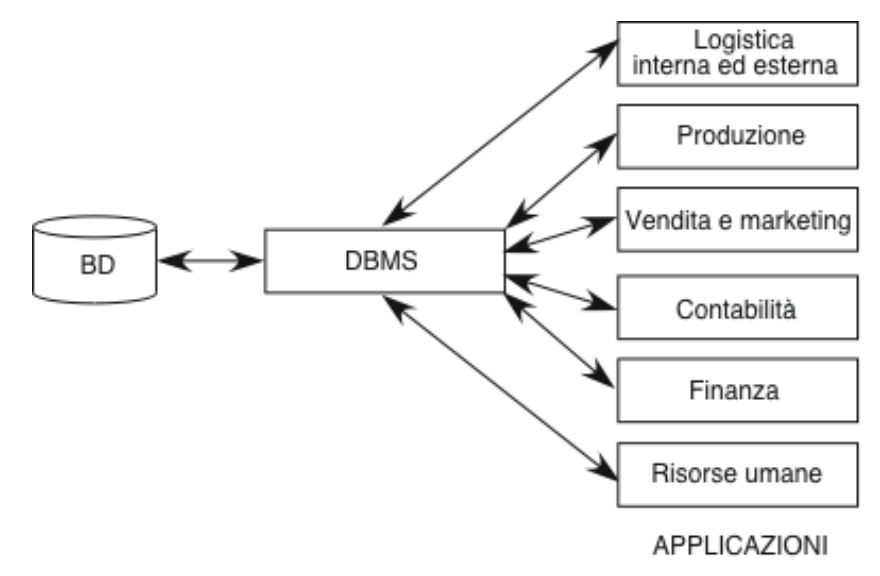
\includegraphics[width=0.6\textwidth]{immagini/Sistema_informatico_operativo.png}
\end{figure}

\subsubsection{Elaborazioni su BD:\ OLTP (On-Line Transaction Processing) \\Sistemi transazionali}
Uso principale dei DBMS.\
Tradizionale elaborazione di transazioni, che realizzano i processi operativi per il funzionamento di organizzazioni:
\begin{itemize}
	\item operazioni predefinite e relativamente semplici;
	\item ogni operazione coinvolge ``pochi'' dati;
	\item dati di dettaglio, aggiornati.
\end{itemize}

\subsection{Sistemi informatici direzionali}

I dati sono organizzati in Data Warehouse (DW) e gestiti da un opportuno sistema.\
Le applicazioni, dette di \textit{business intelligence}, sono strumenti di supporto ai processi di controllo delle prestazioni aziendali e di decisione manageriale.

\begin{figure}[H]
	\centering
	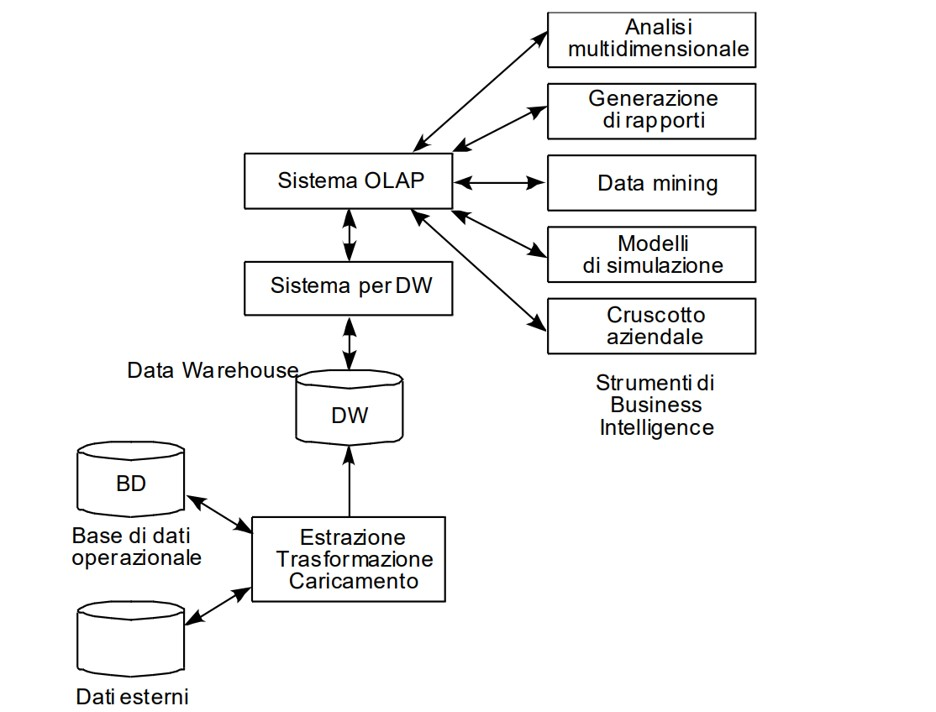
\includegraphics[width=0.8\textwidth]{immagini/Sistema_informatico_direzionale.jpg}
\end{figure}
\subsubsection{Elaborazioni su DW:\ OLAP (On-Line Analytical Processing)}

Uso principale dei \textbf{data warehouse}:
\begin{itemize}
	\item analisi dei dati di supporto alle decisioni;
	\item operazioni complesse e casuali;
	\item ogni operazione può coinvolgere molti dati;
	\item dati aggregati, storici, anche non attualissimi.
\end{itemize}

\begin{table}[H]
	\centering
	\begin{tabular}{|m{8em}|l|l|}
		\hline
		                                       & \textbf{OLTP}          & \textbf{OLAP}                \\\hline
		\textbf{Scopi}                         & Supporto operatività   & Supporto decisioni           \\\hline
		\textbf{Utenti}                        & Molti, esecutivi       & Pochi, dirigenti e analisti  \\\hline
		\textbf{Dati}                          & Analitici, relazionali & Sintetici, multidimensionali \\\hline
		\textbf{Usi}                           & Noti a priori          & Poco prevedibili             \\\hline
		\textbf{Quantità di dati per attività} & Bassa (decine)         & Alta (milioni)               \\\hline
		\textbf{Orientamento}                  & Applicazione           & Soggetto                     \\\hline
		\textbf{Aggiornamenti}                 & Frequenti              & Rari                         \\\hline
		\textbf{Visione dei dati}              & Corrente               & Storica                      \\\hline
		\textbf{Ottimizzati pe}r               & Transazioni            & Analisi dei dati             \\\hline
	\end{tabular}
	\caption*{Differenze tra OLTP e OLAP}
\end{table}

\section{Analisi dei dati}

Dati \textbf{aggregati}:\ non interessa un dato, ma la somma, la media, il minimo, il massimo di una misura.

Presentazione \textbf{multidimensionale}:\ interessa incrociare le informazioni per analizzarle da punti di vista diversi e valutare i risultati del business per intervenire sui problemi critici o per cogliere nuove opportunità.

Analisi a \textbf{diversi livelli di dettaglio}, per esempio una volta scoperto un calo delle vendite in un determinato periodo in una regione specifica, si passa ad un'analisi dettagliata nell'area di interesse per cercare di scoprire le cause (dimensioni con gerarchie).

\subsubsection{Big Data}

Big Data è un termine ampio, riferito a situazioni in cui l'approccio ``schema-first'' tipico di DB o DW risulta troppo restrittivo o troppo lento.\
Le tre \textit{V}:\ \textit{v}olume, \textit{v}arietà e \textit{v}elocità.\

I Big Data sono in genere associati a sistemi NoSQL, Machine Learning e approccio Data Lake.

\section{Sistemi per basi di dati (Data Base Management Systems - DBMS)}

\begin{definition}
	Un DBMS è un sistema centralizzato o distribuito che offre op\-portuni linguaggi per:\
	\begin{itemize}
		\item definire lo \textbf{schema} di una basi di dati (lo schema va definito prima di creare dati);
		\item scegliere le \textbf{strutture dati} per la memorizzazione dei dati;
		\item memorizzare i dati rispettando i \textbf{vincoli} definiti nello schema;
		\item recuperare e modificare i dati interattivamente (linguaggio di interrogazione o \textbf{query language}) o da programmi.
	\end{itemize}
\end{definition}

\subsection{Architettura dei DBMS centralizzati}

Una base di dati è una raccolta di dati permanenti suddivisi in due categorie.\
I \textbf{metadati} descrivono fatti sullo schema dei dati, utenti autorizzati, applicazioni, parametri quantitativi sui dati, \dots; sono descritti da uno
schema usando il modello dei dati adottato dal DBMS e sono interrogabili con le stesse modalità previste per i dati.\
I \textbf{dati} sono le rappresentazioni di certi fatti conformi alle definizioni dello schema, con le seguenti caratteristiche:
\begin{itemize}
	\item sono organizzati in \textbf{insiemi strutturati e omogenei} fra i quali sono definite delle \textbf{relazioni}.\ La struttura dei dati e le relazioni sono descritte nello schema usando i meccanismi di astrazione del modello dei dati del DBMS;
	\item sono \textbf{molti}, in assoluto e rispetto ai metadati, e non possono essere gestiti in memoria temporanea;
	\item sono accessibili mediante \textbf{transazioni}, unità di lavoro atomiche che non possono avere effetti parziali;
	\item sono \textbf{protetti} sia da accesso da parte di utenti non autorizzati, sia da corruzione dovuta a malfunzionamenti hardware e software;
	\item sono utilizzabili \textbf{contemporaneamente} da utenti diversi.
\end{itemize}
Il \textbf{modello relazionale} dei dati è il più diffuso fra i DBMS commerciali.\
Il meccanismo di astrazione fondamentale è la \textbf{relazione} (\textbf{tabella}), sostanzialmente un insieme di record con campi elementari; lo schema di una relazione ne definisce il nome e descrive la struttura dei possibili elementi della relazione (insieme di attributi con il loro tipo).

\subsection{Funzionalità dei DBMS}

\begin{itemize}
	\item Linguaggio per la definizione della base di dati;
	\item Linguaggi per l'uso dei dati;
	\item Meccanismi per il controllo dei dati;
	\item Strumenti per il responsabile della base di dati;
	\item Strumenti per lo sviluppo delle applicazioni.
\end{itemize}

\subsubsection{Linguaggio per la definizione della base di dati (DDL)}

È utile distinguere tre diversi livelli di descrizione dei dati (schemi):\ il livello di vista logica, il livello logico e quello fisico.
\begin{figure}[H]
	\centering
	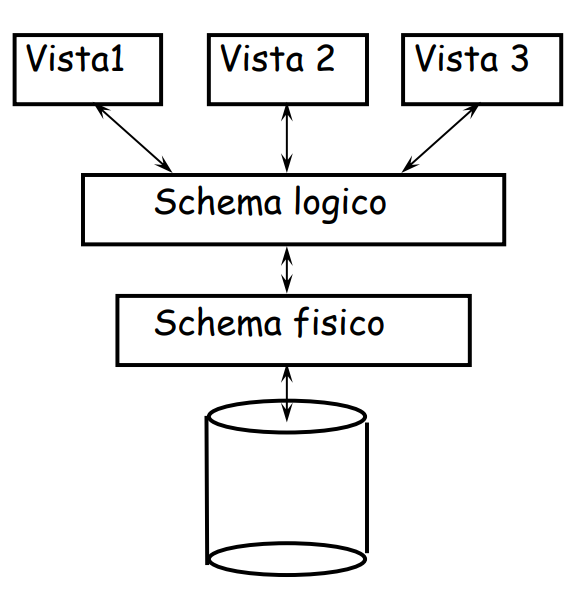
\includegraphics[width=0.3\textwidth]{immagini/livelli_descrizione_dati.png}
\end{figure}
\noindent\textbf{Livello logico}:\ descrive la struttura degli insiemi di dati e delle relazioni fra loro, secondo un certo modello dei dati, senza nessun riferimento alla loro organizzazione fisica nella memoria permanente (schema logico).

\noindent\textbf{Livello fisico}:\ descrive come vanno organizzati fisicamente i dati nelle memorie permanenti e quali strutture dati ausiliarie prevedere per facilitarne l'uso (schema fisico o interno).

\noindent\textbf{Vista logica}:\ descrive come deve apparire la struttura della base di dati ad una certa applicazione (schema esterno o vista).

L'approccio con tre livelli di descrizione dei dati è stato proposto come un modo per garantire le \textbf{proprietà di indipendenza logica e fisica dei dati}, che sono fra gli obiettivi più importanti dei DBMS.
\begin{itemize}
	\item \textbf{Indipendenza fisica}:\ i programmi applicativi non devono essere modificati in seguito a modifiche dell'organizzazione fisica dei dati.
	\item \textbf{Indipendenza logica}:\ i programmi applicativi non devono essere modificati in seguito a modifiche dello schema logico.
\end{itemize}

\subsubsection{Linguaggi per l'uso dei dati}

Un \textbf{DBMS} deve prevedere \textbf{più modalità d'uso} per soddisfare le esigenze delle diverse categorie di utenti che possono accedere alla base di dati (dati e catalogo):
\begin{itemize}
	\item Un'interfaccia grafica per accedere ai dati
	\item Un linguaggio di interrogazione per gli utenti non programmatori
	\item Un linguaggio di programmazione per gli utenti che sviluppano applicazioni:
	      \begin{itemize}
		      \item integrazione DDL e DML nel linguaggio ospite:\ procedure predefinite, estensione del compilatore, precompilazione
		      \item comunicazione tra linguaggio e DBMS
	      \end{itemize}
	\item Un linguaggio per lo sviluppo di interfacce per le applicazioni
\end{itemize}

\subsubsection{Strumenti}

\textbf{Strumenti per l'amministratore} della base di dati
\begin{itemize}
	\item Un linguaggio per la definizione e la modifica degli schemi logico, interno ed esterno.
	\item Strumenti per il controllo e messa a punto del funzionamento del sistema.
	\item Strumenti per stabilire i diritti di accesso ai dati e per ripristinare la base di dati in caso di malfunzionamenti.
\end{itemize}
\textbf{Strumenti per lo sviluppo} delle applicazioni
\begin{itemize}
	\item Produzione di rapporti, grafici, fogli elettronici
	\item Sviluppo di menù, forme, componenti grafici
\end{itemize}

\subsubsection{Linguaggi per le basi di dati}

Disponibilità di vari linguaggi e interfacce diverse:\ linguaggi testuali interattivi (es.\ SQL), comandi (come quelli del linguaggio interattivo) immersi in un linguaggio ospite (es.\ C, Cobol, etc.), comandi (come quelli del linguaggio interattivo) immersi in un linguaggio ad hoc (es.\ PL/SQL) con  altre funzionalità e anche con l'ausilio di strumenti di sviluppo, interfacce amichevoli (senza linguaggio testuale).

\subsubsection{Schemi e istanze}
In ogni base di dati si distinguono:\ \textit{lo \textbf{schema}, sostanzialmente invariante nel tempo, che ne descrive la struttura (aspetto intensionale)}, ovvero le intestazioni delle tabelle, e  \textit{l'\textbf{istanza}, i valori attuali, che possono cambiare anche molto rapidamente (aspetto estensionale)}, cioè il ``corpo'' di ciascuna tabella.

Nei linguaggi di interrogazione di basi di dati distinguiamo tra

\begin{itemize}
	\item \textbf{Data Manipulation Language} (\textbf{DML}):\ per l'interrogazione e l'aggiornamento di (istanze di) basi di dati.
	\item \textbf{Data Definition Language} (\textbf{DDL}):\ per la definizione di schemi (logici, esterni, fisici) e altre operazioni generali.
\end{itemize}

\subsubsection{Meccanismi per il controllo dei dati}

Una caratteristica molto importante dei DBMS è il tipo di meccanismi offerti per garantire le seguenti proprietà di una base di dati:
\begin{itemize}
	\item \textbf{Integrità}:\ mantenimento delle proprietà specificate in modo dichiarativo nello schema (vincoli d'integrità).
	\item \textbf{Sicurezza}:\ protezione dei dati da usi non autorizzati.
	\item \textbf{Affidabilità}:\ protezione dei dati da malfunzionamenti hardware o software (fallimenti di transazione, di sistema e disastri) e da interferenze indesiderate dovute all'accesso concorrente ai dati da parte di più utenti.
\end{itemize}

\begin{definition}

	Una \textbf{transazione} è una sequenza di azioni di lettura e scrittura in memoria permanente e di elaborazioni di dati in memoria temporanea, con le seguenti proprietà:
	\begin{itemize}
		\item \textbf{Atomicità}:\ le transazioni che terminano in modo prematuro (\textit{aborted transactions}) sono trattate dal sistema come se non fossero mai iniziate; pertanto eventuali loro effetti sulla base di dati sono annullati.
		\item \textbf{Serializzabilità}:\ nel caso di esecuzioni concorrenti di più transazioni, l'effetto complessivo è quello di una esecuzione seriale.
		\item \textbf{Persistenza}:\ le modifiche sulla base di dati di una transazione terminata normalmente sono permanenti, cioè non sono alterabili da eventuali malfunzionamenti.
	\end{itemize}
\end{definition}

\subsection{Conclusione}

Un \textbf{DataBase Management System} (\textbf{DBMS}) è un sistema (\textit{prodotto software}) in grado di gestire \textit{collezioni di dati} che siano (anche) \textbf{grandi}, \textbf{persistenti} (con un periodo di vita indipendente dalle singole esecuzioni dei programmi che le utilizzano) e \textbf{condivise} (utilizzate da applicazioni diverse), garantendo \textbf{affidabilità} (resistenza a malfunzionamenti hardware e software-recovery) e \textbf{privatezza} (con una disciplina e un controllo degli accessi).\
Come ogni prodotto informatico, un DBMS deve essere \textbf{efficiente} (utilizzando al meglio le risorse di spazio e tempo del sistema)
ed \textbf{efficace} (rendendo produttive le attività dei suoi utilizzatori).

\noindent \textbf{Vantaggi}
\begin{itemize}
	\item Indipendenza dei dati
	\item Recupero efficiente dei dati
	\item Integrità e sicurezza dei dati
	\item Accessi interattivi, concorrenti e protetti dai malfunzionamenti
	\item Amministrazione dei dati
	\item Riduzione dei tempi di sviluppo delle applicazioni
	\item La riduzione dei costi della tecnologia e i possibili tipi di DBMS disponibili sul mercato facilitano la loro diffusione.
\end{itemize}
\textbf{Svantaggi}
\begin{itemize}
	\item Prima di caricare i dati è necessario definire uno schema
	\item Possono essere costosi e complessi da installare e mantenere in esercizi
	\item Possono gestire solo dati strutturati e omogenei
	\item Sono ottimizzati per le applicazioni OLTP, non per quelle OLAP
\end{itemize}
